%%%%%%%%%%%%%%%%%%%%%%%%%%%%%%%%%%%%%%%%%%%%%%%%%%%%%%%%%%%%%%%
%
% Welcome to Overleaf --- just edit your LaTeX on the left,
% and we'll compile it for you on the right. If you open the
% 'Share' menu, you can invite other users to edit at the same
% time. See www.overleaf.com/learn for more info. Enjoy!
%
%%%%%%%%%%%%%%%%%%%%%%%%%%%%%%%%%%%%%%%%%%%%%%%%%%%%%%%%%%%%%%%
% --------------------------------------------------------------
% Homework Template by Dana Ernst, reproduced here with thanks.
% --------------------------------------------------------------
% This is all preamble stuff that you don't have to worry about.
% Head down to where it says "Start here"
% --------------------------------------------------------------

\documentclass[12pt]{article}
\usepackage{titlesec}

\usepackage[margin=1in]{geometry} 
\usepackage{amsmath,amsthm,amssymb}
\usepackage{cite}
\usepackage{graphicx}

\newcommand{\N}{\mathbb{N}}
\newcommand{\Z}{\mathbb{Z}}

\newcommand{\Eqref}[1]{Eq.~\eqref{#1}}
\newcommand{\Figref}[1]{Fig.~\ref{#1}}

% this improves readability of to-do notes
\setlength{\marginparwidth}{2.20cm}
\usepackage[color=green!60]{todonotes}
\newcommand{\tde}[1]{\todo[color=blue!20]{\footnotesize #1 \\--ECD}}
\newcommand{\tdei}[1]{\todo[inline,color=blue!20]{\footnotesize #1 --ECD}}

\newenvironment{theorem}[2][Theorem]{\begin{trivlist}
\item[\hskip \labelsep {\bfseries #1}\hskip \labelsep {\bfseries #2.}]}{\end{trivlist}}
\newenvironment{lemma}[2][Lemma]{\begin{trivlist}
\item[\hskip \labelsep {\bfseries #1}\hskip \labelsep {\bfseries #2.}]}{\end{trivlist}}
\newenvironment{exercise}[2][Exercise]{\begin{trivlist}
\item[\hskip \labelsep {\bfseries #1}\hskip \labelsep {\bfseries #2.}]}{\end{trivlist}}
\newenvironment{problem}[2][Problem]{\begin{trivlist}
\item[\hskip \labelsep {\bfseries #1}\hskip \labelsep {\bfseries #2.}]}{\end{trivlist}}
\newenvironment{question}[2][Question]{\begin{trivlist}
\item[\hskip \labelsep {\bfseries #1}\hskip \labelsep {\bfseries #2.}]}{\end{trivlist}}
\newenvironment{corollary}[2][Corollary]{\begin{trivlist}
\item[\hskip \labelsep {\bfseries #1}\hskip \labelsep {\bfseries #2.}]}{\end{trivlist}}

\begin{document}

% --------------------------------------------------------------
%                         Start here
% --------------------------------------------------------------

\title{Testing if CRBM kernels learn Ising symmetries}%replace X with the appropriate number
\author{Emanuel Casiano-Diaz}
\maketitle

In order to understand if the kernel of the CRBM learns the symmetries of the physical model (which in this case will be the $2D$ Ising Model) even when the kernel is not explicitly symmetrized, we performed a set of numerical tests.

% --------------------------------------------------------------
\section{Test: Learned kernels for original vs rotated training set}

For this test, we train an RBM using a set of completely random visible layer configurations (i.e, they were not sampled from Monte Carlo nor they represent the full set of possible spin configurations). Additionally, the kernels were initialized to a shape that looked similar to what we have noticed that the CRBM learns, which is that all weights are zero, except three of them that form an ``L"-shaped configuration. In this ``L"-shaped configuration, the ``elbow" consists of a weight that is larger in magnitude than the other two. 

After the CRBM was trained using the original set of visible layer configurations, we proceeded to generate the exact same data set, but with each of the configurations rotated by $90^\circ$ clockwise. 

If the learned weights on both cases were the same, this might suggest that the CRBM kernel is indeed learning the symmetries of the physical model, even in the absence of an explicit kernel symmetrization subroutine in the training loop.

\Figref{fig:2by2_kernels_heatmap} shows the learned kernels. For this example, we chose two kernels of size $2\time2$ each. In the figure, the top two kernels were learned using the original data set while the bottom was learned using the same data set but rotated 90 degrees clockwise. Upon closer inspection, it seems like in both cases, the weights were indeed roughly for the original and rotated training set, although their positions on the kernels might have changed. This is evidenced by the positions of the top right and bottom left weights having swapped with each other.To see this more clearly, the numeric values of the learned kernels can be seen in \Figref{fig:2by2_kernels_numeric}


%%%%%%%%%%%%%%%%%%%%%%%%%%%%%%%%%%%%%%%%%%%%%%%%%%
\begin{figure}[t!]
\begin{center}
    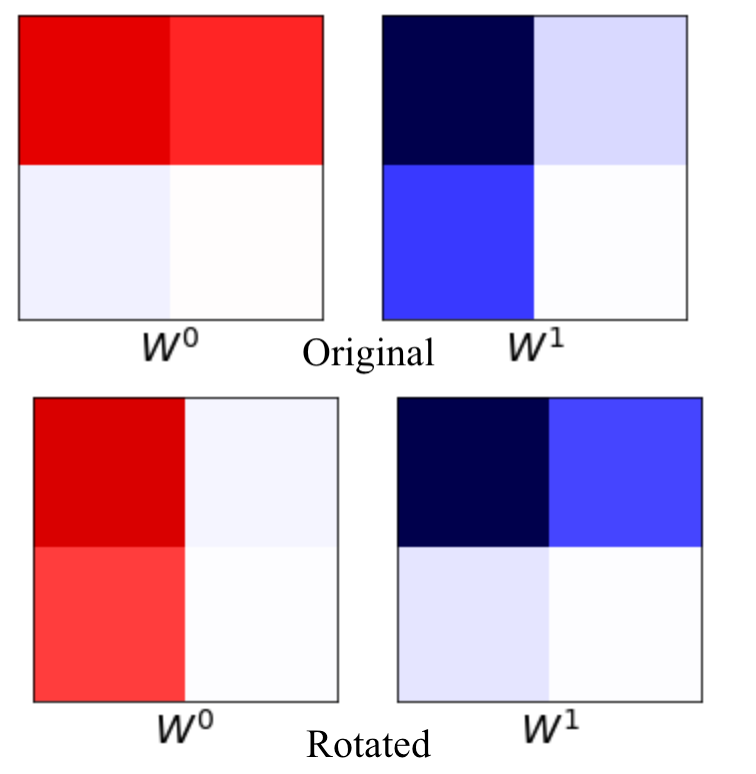
\includegraphics[width=1.0\columnwidth]{figures/learned_kernels_2by2_combined_heatmap.png}
\end{center}
\caption{Heatmap of learned kernels. The top two kernels show the learned weights for the case in which the CRBM was trained using the original data set. The bottom kernel corresponds to the case of the rotated data set. The colors seem to suggest that the learned weights in both cases were roughly the same, with the only difference being that the top-right and bottom-left weights are swapped.}
\label{fig:2by2_kernels_heatmap}
\end{figure}
%%%%%%%%%%%%%%%%%%%%%%%%%%%%%%%%%%%%%%%%%%%%%%%%%%

%%%%%%%%%%%%%%%%%%%%%%%%%%%%%%%%%%%%%%%%%%%%%%%%%%
\begin{figure}[t!]
\begin{center}
    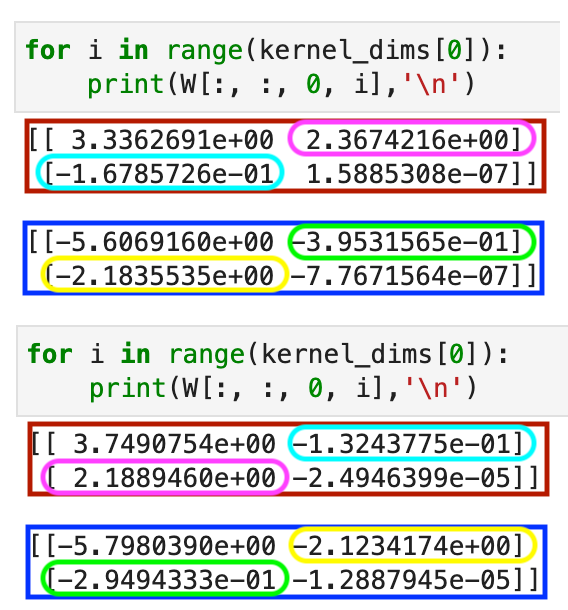
\includegraphics[width=1.0\columnwidth]{figures/learned_kernels_2by2_combined_numeric.png}
\end{center}
\caption{Numeric values of learned kernels for original (top) and rotated (bottom) data sets. Color coded ovals are used to match the weights that seemingly swapped positions after training with the rotated data set.}
\label{fig:2by2_kernels_numeric}
\end{figure}
%%%%%%%%%%%%%%%%%%%%%%%%%%%%%%%%%%%%%%%%%%%%%%%%%%

The results potentially suggest that the ``L"-shaped patterns correspond to kernels that have learned the symmetries of the Ising model.

% --------------------------------------------------------------
\newcommand{\sectionbreak}{\clearpage}
\section{Test: Free-energy for non-symmetrized vs symmetrized kernels}

Recall that we want the free-energy of the visible layer of the CRBM to match the physical distribution of the model:
%
\begin{align}
P(v) &= P(\sigma) \nonumber \\
 \frac{1}{\mathcal{Z}_{\rm{CRBM}}} e^{-F(v)} &= \frac{1}{\mathcal{Z}_{\rm{phys}}} e^{-E(\sigma)},
\end{align}
%
which is equivalent to saying that the free-energy $F(v)$ and the physical energy $E(\sigma)$ should be equal, up to an additive constant:
%
\begin{equation}
E(\sigma) = F(v) + \log \left ( \frac{\mathcal{Z}_{\rm{CRBM}}}{\mathcal{Z}_{\rm{phys}}} \right ) \equiv F(v) + C
\end{equation}
%
Since the free and physical energies are the same, up to a constant, and the physical energy is invariant under reflection and rotation symmetries, the free-energy should also be invariant under these symmetries. 

\tdei{Still need to perform this test. Go to next section :)}

% --------------------------------------------------------------
\section{Test: What free-energy do non-symmetrized vs symmetrized kernels learn?}

We were thinking that, for reasons that are not clear yet, both the ``L"-shaped and the explicitly symmetrized kernels are encoding the same information about the symmetries. 

To test this, we trained two CRBMs on the same data set. For one of them, the rotation and reflection symmetrizations were performed explicitly on the kernel at regular intervals in the training loop, while for the other CRBM, the kernel was not explicitly symmetrized. The learned kernels can be seen in \Figref{fig:symm_vs_nonSymm_heatmaps}. The ``L"-shaped kernel is for the case of no explicit symmetrization and the cross-shaped kernel has been explicitly symmetrized for reflection and rotation. The non-zero weights of the symmetrized kernel vs the non-symmetrized one seem to differ by a factor of 2. Interestingly, for the heavy weight, the symmetrized one is roughly doubled. But, for the lighter weights, the symmetrized ones are instead halved.

%%%%%%%%%%%%%%%%%%%%%%%%%%%%%%%%%%%%%%%%%%%%%%%%%%
\begin{figure}[h!]
\begin{center}
    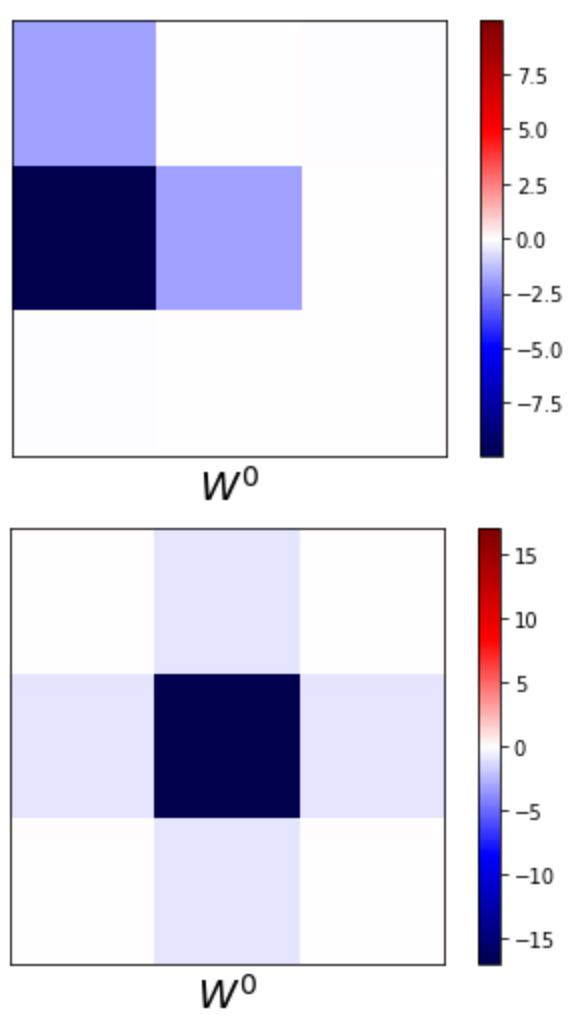
\includegraphics[width=0.5\columnwidth]{figures/learned_kernel_3by3_combined_heatmap_nonSymmVsSymm.png}
\end{center}
\caption{Learned kernels with no explicit symmetrization (top) and with explicit rotation and reflection symmetrization (bottom).}
\label{fig:symm_vs_nonSymm_heatmaps}
\end{figure}
%%%%%%%%%%%%%%%%%%%%%%%%%%%%%%%%%%%%%%%%%%%%%%%%%%


\Figref{fig:symm_vs_nonSymm_free_energies} shows the free-energies computed for a fixed set of random configurations of the visible layer. The top result is with no explicit symmetrization of the kernel, while the bottom one is with explicit symmetrization. Notice that up to constant factor, the free-energies are the same. Thus, the free-energy is invariant under symmetrization of the kernel. Somehow, the cross and ``L"-shaped kernels are encoding the same information.

We are not sure yet if this is a consequence of the simplicity of the Ising model or if both representations are somehow equivalent to each other.

%%%%%%%%%%%%%%%%%%%%%%%%%%%%%%%%%%%%%%%%%%%%%%%%%%
\begin{figure}[h!]
\begin{center}
    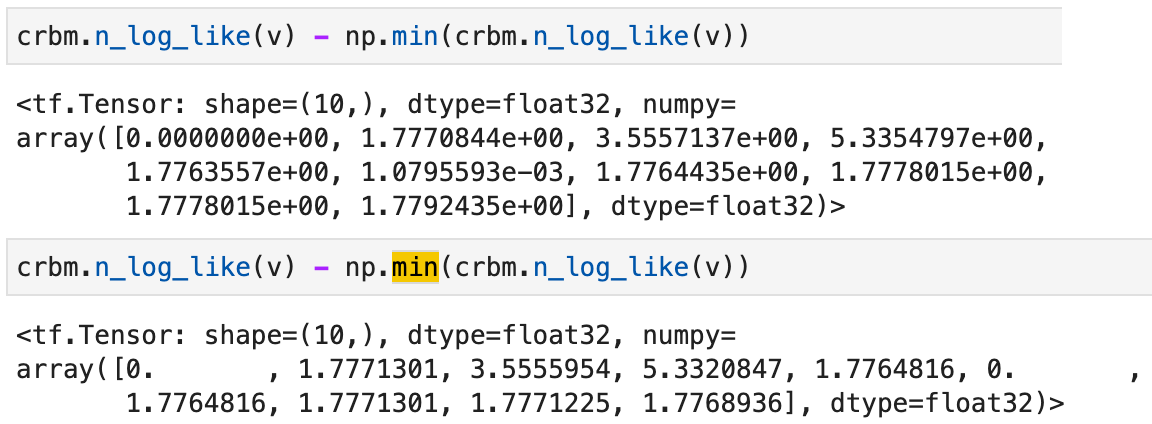
\includegraphics[width=1.0\columnwidth]{figures/symmetrizedVSnonSymm_free_energies.png}
\end{center}
\caption{Learned kernels with no explicit symmetrization (top) and with explicit rotation and reflection symmetrization (bottom).}
\label{fig:symm_vs_nonSymm_free_energies}
\end{figure}
%%%%%%%%%%%%%%%%%%%%%%%%%%%%%%%%%%%%%%%%%%%%%%%%%%

\section{Moving forward}

It does not seem like implementing the explicit symmetrization will give much benefit in the case of the zero-field, nearest-neighbor Ising model. Some potential avenues of study could instead be to implement the sampler that Sakib suggested, or to study a more complicated model in which explicitly implementing the symmetries might provide more benefit.

% --------------------------------------------------------------

% --------------------------------------------------------------
%     You don't have to mess with anything below this line.
% --------------------------------------------------------------


\bibliographystyle{plain}
\bibliography{refs}

\end{document}